%-------------------------------------------
\begin{frame}[containsverbatim]
\frametitle{Snakemake point}
%-------------------------------------------
\begin{block}{So far, we've seen:}
\begin{itemize}
    \item the rule and the workflow concepts, the snakefile
    \item how rules are linked thank to input/output files and the first rule, the target rule
    \item how to generalize the inputs of a rule using wildcards on filenames (and the \verb|expand| function)
    \item how to redirect \verb|stdout| and \verb|stderr| streams (log)
\end{itemize}
\end{block}
\begin{block}{From now, we will seen some snakemake options:}
\begin{itemize}
    \item adding a configuration file
    \item getting file names from the file system
    \item use a conda environment
    \item to visualize the workflow diagram, use a dry-run option, etc
    %\item \alert{the container directive ???}
    %\item \alert{how to run snakemake on cluster ???}
\end{itemize}
\end{block}
\end{frame}
%-------------------------------------------
\begin{frame}[containsverbatim]
\frametitle{Using a configuration file}
%-------------------------------------------
Why use a configuration file?\\
To place all hard-coding values of the snakefile (paths to files, core numbers, parameter values, etc)
\begin{block}{How to?}
\begin{itemize}
    \item create a file written in yml or json (eg. \verb|myConfig.yml|)
    \item run with the \verb|--configfile myConfig.yml| Snakemake option or ii) add \verb|configfile: myConfig.yml| at the beginning of the snakefile
    \item in the snakefile, call the defined items with \verb|config["item1"]|
\end{itemize}
\end{block}
\end{frame}
%-------------------------------------------
\begin{frame}[containsverbatim]
\frametitle{Using a configuration file}
%-------------------------------------------
\begin{exampleblock}{myConfig.yml}
\begin{lstlisting}
dataDir:
  Data/
\end{lstlisting}
\end{exampleblock}
\begin{exampleblock}{Replace "Data/..." in inputs by a config call:}
\begin{lstlisting}
rule fastqc:   
   input: config["dataDir"]+"{sample}.fastq.gz"
\end{lstlisting}
\end{exampleblock}
\begin{exampleblock}{And Run with the configfile option:}
\begin{lstlisting}
snakemake -c1 -s ex1_o7.smk --configfile myConfig.yml
\end{lstlisting}
\end{exampleblock}
\end{frame}
%-------------------------------------------
\begin{frame}[containsverbatim]
\frametitle{File names from the file system}
%-------------------------------------------
To deduce the identifiers (eg. IDs) of files in a directory, use the inbuilt \verb|glob_wildcards| function:
\begin{block}{Eg. of the glob$\_$wilcards function}
\begin{lstlisting}
IDs, = glob_wildcards("dirpath/{id}.fastq")
\end{lstlisting}
\end{block}
\verb|glob_wildcards()| matches the given pattern against the files present in the file system and thereby infers the values for all wildcards in the pattern (\verb|{id}| here). 
\vfill
Don't forget the \textcolor{blue}{coma} after the name (left hand side, \verb|IDs| here).
\end{frame}
%-------------------------------------------
\begin{frame}[containsverbatim]
\frametitle{Conda environment}
%-------------------------------------------
\begin{block}{Snakemake and conda}
In the practical exercise we will have one conda environment for executing the whole Snakemake workflow. \\
Snakemake also supports using explicit conda environments on a per-rule basis:
\begin{itemize}
    \item add a \verb|conda:| directive in the rule definition :
\begin{lstlisting}
    conda: rule-specific-env.yml
\end{lstlisting}
    \item run Snakemake with the \verb|--use-conda| option
\end{itemize}
The specified environment will be created and activated on the fly by Snakemake and the rule will then be run in the conda environment.
\end{block}
\end{frame}
%-------------------------------------------
\begin{frame}[containsverbatim]
\frametitle{Snakemake DAG visualization}
%-------------------------------------------
\begin{block}{}
Snakemake uses \verb|dot| tool (from graphviz package) to create diagrams of the complete workflow (\verb|--dag|) or the rules dependencies (\verb|--rulegraph|):
\begin{lstlisting}
snakemake --dag -s ex1_o7.smk | dot -Tpng > ex1_o7_dag.png
snakemake --rulegraph -s ex1_o7.smk | dot -Tpng > ex1_o7_rule.png
\end{lstlisting}
\end{block}
\begin{columns}
 \column{0.80\textwidth}
   \begin{center}
   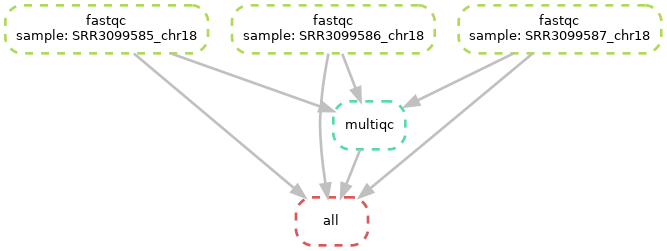
\includegraphics[height=3.6cm]{03_workflow/images/ex1_o7_dag.png}
   \end{center}
 \column{0.20\textwidth}
    \begin{center}
    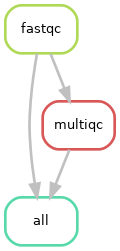
\includegraphics[height=3.6cm]{03_workflow/images/ex1_o7_rule.png}
    \end{center}
\end{columns}
\end{frame}
%-------------------------------------------
\begin{frame}[containsverbatim]
\frametitle{Other useful options}
%-------------------------------------------
\begin{block}{Running options}
\begin{itemize}
    \item dry-run, do not execute anything, display what would be done: \verb|-n --dryrun|
    \item print the shell command: \verb|-p --printshellcmds |
    \item print the reason for each rule execution: \verb|-r --reason|
    \item print a summary and status of rule: \verb|-D|
    \item limit the number of jobs in parallel: \verb|-j 1| (cores: \verb|-c 1|)
    \item automatically create HTML reports (\verb|--report report.html|) containing runtime statistics, a visualization of the workflow topology, used software and data provenance information (need to add the \verb|jinja2| package as a dependency)
\end{itemize}
\end{block}
\vfill
\href{https://snakemake.readthedocs.io/en/stable/executing/cli.html#all-option}{\textcolor{blue}{\underline{all Snakemake options}}}
\end{frame}


%-------------------------------------------
%\begin{frame}[containsverbatim]
%\frametitle{IFB cluster options}
%-------------------------------------------
%\begin{block}{interactive session}
%To use the option \verb|--cores=2|, don't forget to ask 2 CPUS for the interactive session (\verb|sinteractive --cpus=2|)
%\end{block}
%\begin{block}{cluster mode}
%To launch the snakefile on a cluster mode, just do:
%\begin{itemize}
%    \item load the \verb|slurm-drmaa| module
%    \item run snakemake with the \verb|--drmaa| option
%\begin{lstlisting}
%snakemake --drmaa --jobs=12 -s ex2_o6.smk --configfile ex2_o1.yml
%\end{lstlisting}
%\end{itemize}
%\end{block}
%\end{frame}
